\documentclass{ximera}


\graphicspath{
  {./}
  {ximeraTutorial/}
  {basicPhilosophy/}
}

\newcommand{\mooculus}{\textsf{\textbf{MOOC}\textnormal{\textsf{ULUS}}}}

\usepackage{tkz-euclide}\usepackage{tikz}
\usepackage{tikz-cd}
\usetikzlibrary{arrows}
\tikzset{>=stealth,commutative diagrams/.cd,
  arrow style=tikz,diagrams={>=stealth}} %% cool arrow head
\tikzset{shorten <>/.style={ shorten >=#1, shorten <=#1 } } %% allows shorter vectors

\usetikzlibrary{backgrounds} %% for boxes around graphs
\usetikzlibrary{shapes,positioning}  %% Clouds and stars
\usetikzlibrary{matrix} %% for matrix
\usepgfplotslibrary{polar} %% for polar plots
\usepgfplotslibrary{fillbetween} %% to shade area between curves in TikZ
\usetkzobj{all}
\usepackage[makeroom]{cancel} %% for strike outs
%\usepackage{mathtools} %% for pretty underbrace % Breaks Ximera
%\usepackage{multicol}
\usepackage{pgffor} %% required for integral for loops



%% http://tex.stackexchange.com/questions/66490/drawing-a-tikz-arc-specifying-the-center
%% Draws beach ball
\tikzset{pics/carc/.style args={#1:#2:#3}{code={\draw[pic actions] (#1:#3) arc(#1:#2:#3);}}}



\usepackage{array}
\setlength{\extrarowheight}{+.1cm}
\newdimen\digitwidth
\settowidth\digitwidth{9}
\def\divrule#1#2{
\noalign{\moveright#1\digitwidth
\vbox{\hrule width#2\digitwidth}}}






\DeclareMathOperator{\arccot}{arccot}
\DeclareMathOperator{\arcsec}{arcsec}
\DeclareMathOperator{\arccsc}{arccsc}

















%%This is to help with formatting on future title pages.
\newenvironment{sectionOutcomes}{}{}


\title{Length}

\begin{document}

\begin{abstract}
rate, length, and time
\end{abstract}
\maketitle




\begin{center}
\textbf{\textcolor{purple!85!blue}{Distance = Rate $\cdot$ Time}} 
\end{center}

This relationship is extremely common in our situations.  We might see it as



\begin{center}
\textbf{\textcolor{purple!85!blue}{Length = Rate $\cdot$ Time}} 
\end{center}



However, these are not exactly correct.  The relationship is not between distance and time.  The rate is a comparison measurement between \textcolor{red!80!black}{change in length} and \textcolor{red!80!black}{change in time}.



\[
\text{rate} = \frac{\Delta \text{length}}{\Delta \text{time}} = \frac{\Delta \text{distance}}{\Delta \text{time}}
\]

\textbf{Note:} $\Delta$ is our shorthand notation for ``change in''. \\






\subsection{Airplane}

An airplane is flying overhead on a level flight path, 5 miles above the ground.  The plane is travelling at a constant speed and will travel directly over a tracking station. The tracking station's radar antennea measures the distance from the station to the plane.






\textbf{\textcolor{purple!85!blue}{Step 1: A Picture}}


\begin{image}
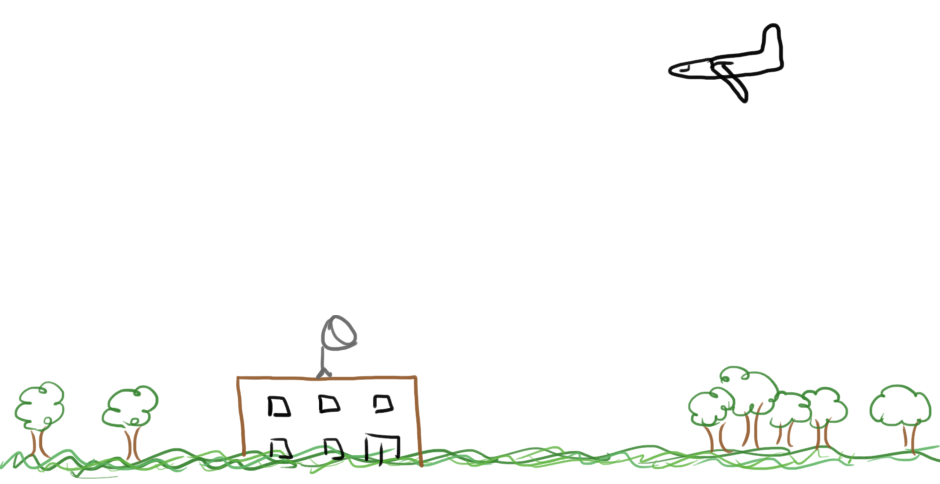
\includegraphics{pics/plane_1.png}
\end{image}




\textbf{\textcolor{purple!85!blue}{Step 2: Identify Measurements}}



\begin{image}
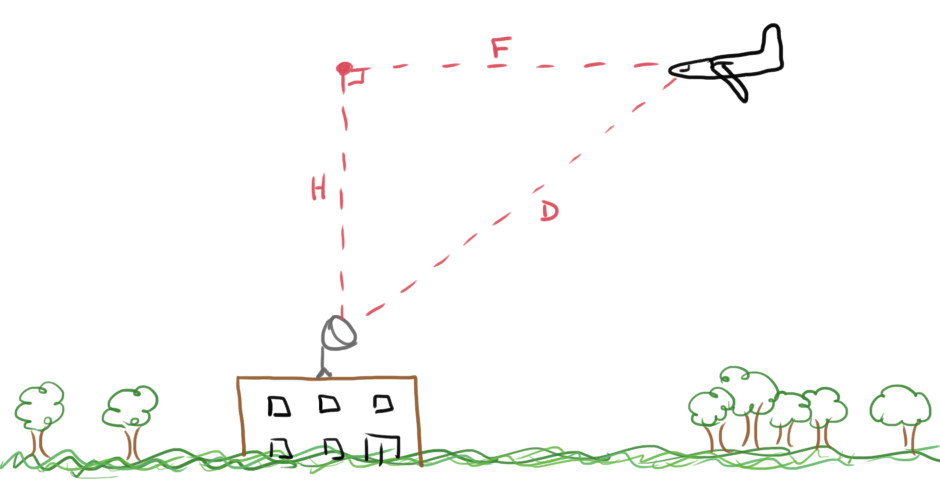
\includegraphics{pics/plane_2.png}
\end{image}



$\blacktriangleright$ We have three pertinent lengths:

\begin{itemize}
\item $D$ is the distance between the station and the plane.
\item $F$ is the flight distance between the plane the point directly above the station.
\item $H$ is the height of the flight path above the station.
\end{itemize}

All of these are functions of time, $t$: $D(t)$, $F(t)$, and $H(t)$.


\begin{question} $\boxdot$ 

Which distance measurement is a constant function?

\begin{multipleChoice}
\choice {$D$}
\choice {$F$}
\choice[correct] {$H$}
\end{multipleChoice}

\end{question}



\begin{question} $\boxdot$ 

Is $D(t)$ an increasing or decreasing function with respect to $t$?

\begin{multipleChoice}
\choice {Increasing}
\choice[correct] {Decreasing}
\end{multipleChoice}

\end{question}



\begin{question} $\boxdot$ 

Is $F(t)$ an increasing or decreasing function with respoect to $t$?

\begin{multipleChoice}
\choice {Increasing}
\choice[correct] {Decreasing}
\end{multipleChoice}

\end{question}










\textbf{\textcolor{purple!85!blue}{Step 3: Geometric Relationships}}


An airplane is flying overhead on a level flight path, 5 miles above the ground.  The plane is travelling at a constant speed and will travel directly over a tracking station. The tracking station's radar antennea measures the distance from the station to the plane. If the distance between the station and the plane is decreasing at a rate of $350$ miles per hour when that distance is $10$ miles, then what is the speed of the plane?


\begin{image}
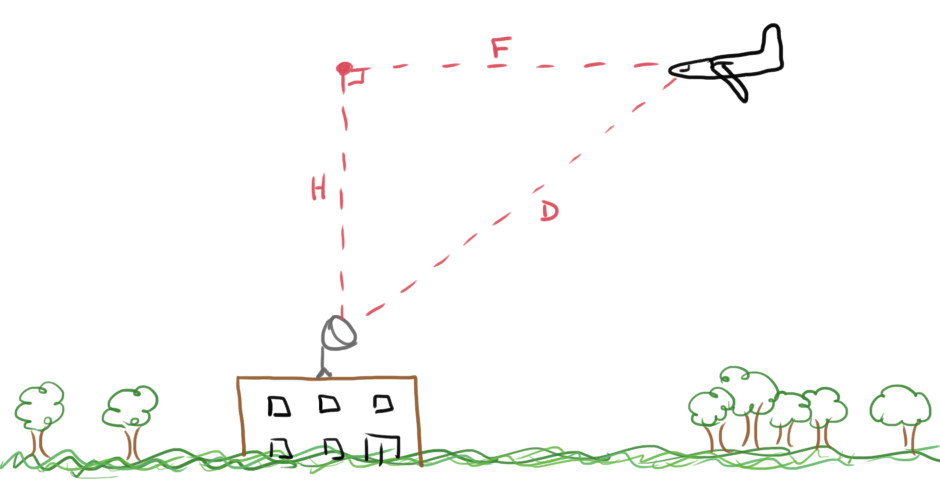
\includegraphics{pics/plane_2.png}
\end{image}





\begin{question} $\boxdot$ 

What geometric shape connects these measurements?

\begin{multipleChoice}
\choice {Rectangle}
\choice[correct] {Right Triangle}
\choice {Circle}
\end{multipleChoice}

\end{question}







\begin{question} $\boxdot$ 

What geometric relationship connects these measurements?

\begin{multipleChoice}
\choice[correct] {Pythagorean Theorem}
\choice {Circumference}
\choice {Similar Triangles}
\end{multipleChoice}

\end{question}






\begin{question} $\boxdot$ 

Which relationship is suggested by the diagram?

\begin{multipleChoice}
\choice {$D^2 + F^2 = H^2$}
\choice[correct] {$H^2 + F^2 = D^2$}
\choice {$H^2 + D^2 = F^2$}
\end{multipleChoice}

\end{question}






\begin{question} $\boxdot$ 

$350$ miles per hour is the rate of change of which measurement?

\begin{multipleChoice}
\choice[correct] {$D$}
\choice {$F$}
\choice {$H$}
\end{multipleChoice}

\end{question}





\end{document}
